\chapter{समतल विद्युत्चुंबकीय तरंगें और ध्रुवण}\label{ch:b2:plane-waves-polarization}

ध्रुवक धूप-चश्मा पहनकर सिर टेढ़ा कीजिए और गीली सड़क की चौंध आती-जाती
रहती है; चश्मे को किसी फ़ोन-पर्दे के सामने घुमाइए और पर्दा काला पड़
जाता है। आपकी आँख तक पहुँचता प्रकाश केवल किसी आवृत्ति और तीव्रता की तरंग
नहीं है: उसकी एक \emph{कंपन-दिशा} भी है, और हर ध्रुवक, पर्दा, त्रि-विम
सिनेमा का लेंस तथा प्रकाशिक तंतु का जोड़ उससे खेलता है। यह अध्याय खाली
आकाश में \omterm{thm:b2:maxwell-equations:maxwell}{मैक्सवेल के समीकरण} हल करता है --- अर्थात् समतल तरंग, जिसके
अनुप्रस्थ विद्युत और चुंबकीय क्षेत्र समकोण पर बँधे हैं --- उन तरंगों के
फैले वर्णक्रम का सर्वेक्षण करता है, और ध्रुवण का अध्ययन करता है: उसका
वर्णन कैसे करें, किसी ध्रुवक से उसे कैसे छाँटें (\omterm{prop:b2:plane-waves-polarization:malus}{मालुस का नियम}), और किसी
द्विअपवर्ती पट्टिका से उसे कैसे बदलें।

\section{निर्वात में समतल तरंगें}

\begin{theorem}[तरंग-समीकरण; समतल प्रगामी संनादी तरंगें]\label{thm:b2:plane-waves-polarization:wave}
\index{विद्युत्चुंबकीय तरंग}\index{समतल तरंग (विद्युत्चुंबकीय)}\index{अनुप्रस्थता}
निर्वात में, जहाँ कोई आवेश और धारा न हो, \omterm{thm:b2:maxwell-equations:maxwell}{मैक्सवेल के समीकरण} ये देते हैं:
\[
\Delta\vect E = \frac1{c^2}\frac{\partial^2\vect E}{\partial t^2} , \qquad
\Delta\vect B = \frac1{c^2}\frac{\partial^2\vect B}{\partial t^2} , \qquad
c = \frac1{\sqrt{\varepsilon_0\mu_0}} = \qty{2.998e8}{m/s} .
\]
\emph{समतल प्रगामी संनादी तरंग} (PPH तरंग) $\underline{\vect E} =
\underline{\vect E}_0\,\eu^{\iu(\omega t - \vect k\cdot\vect r)}$ तब हल है जब
$\omega = ck$ हो (कोई परिक्षेपण नहीं), और तब \omterm{thm:b2:maxwell-equations:maxwell}{मैक्सवेल के समीकरण} यह माँगते हैं:
\[
\vect k\cdot\vect E = 0 , \qquad
\vect B = \frac{\vect k\wedge\vect E}\omega = \frac{\vect u\wedge\vect E}c ,
\]
जहाँ $\vect u = \vect k/k$ संचरण की दिशा है: अर्थात् तरंग
\emph{अनुप्रस्थ} है, $(\vect E, \vect B, \vect u)$ कोई दक्षिण-हस्त लांबिक
त्रिक है, $\vect E$ और $\vect B$ एक ही कला में हैं तथा $B = E/c$। उसकी तीव्रता
$I = \varepsilon_0cE_0^2/2$ है और वह संवेग-अभिवाह $I/c$ ढोती है
(\cref{ch:b2:poynting-vector})।
\end{theorem}

\begin{proof}
\omterm{thm:b2:waves-on-strings:equation}{तरंग-समीकरण} \cref{exo:b2:maxwell-equations:11} में निकाला गया था।
$\eu^{\iu(\omega t - \vect k\cdot\vect r)}$ के लिए $\partial_t \to \iu\omega$ और $\vect\nabla \to
-\iu\vect k$: अतः $\Delta \to -k^2$, इसलिए $k^2 = \omega^2/c^2$; मैक्सवेल--गाउस $-\iu
\vect k\cdot\underline{\vect E} = 0$ देता है, मैक्सवेल--अभिवाह $\vect k\cdot\underline{\vect B} = 0$,
मैक्सवेल--फ़ैराडे $-\iu\vect k\wedge\underline{\vect E} = -\iu\omega\underline{\vect B}$, जिससे
$\underline{\vect B} = \vect k\wedge\underline{\vect E}/\omega$, जिसका मापांक $kE/\omega = E/c$ है और
जो दोनों के लंबवत है; और मैक्सवेल--ऐंपियर तब अपने आप संतुष्ट हो जाता है।
\end{proof}

\begin{omfigure}
\begin{tikzpicture}[font=\small, x=1cm, y=1cm, >=Stealth]
  \draw[->, thick] (-0.3,0) -- (7.4,0) node[right, font=\footnotesize] {$\vect u$};
  \draw[omDef, thick, domain=0:6.8, samples=80] plot (\x,{1.1*cos(deg(1.2*\x))});
  \draw[omProp, thick, domain=0:6.8, samples=80] plot (\x,{-0.4*cos(deg(1.2*\x))});
  \foreach \x in {0,0.65,...,6.6} {
    \pgfmathsetmacro{\e}{1.1*cos(deg(1.2*\x))}
    \draw[omDef, ->] (\x,0) -- (\x,\e);
    \draw[omProp, ->] (\x,0) -- ({\x+0.55*\e*0.36},{-0.4*\e*0.9});
  }
  \node[omDef, font=\footnotesize] at (0.4,1.45) {$\vect E$}; \node[omProp, font=\footnotesize] at (0.9,-0.75) {$\vect B = \vect u\wedge\vect E/c$};
  \draw[<->] (0,-1.3) -- (5.24,-1.3) node[midway, below, font=\footnotesize] {$\lambda = 2\pi/k = c/f$};
\end{tikzpicture}

{\small किसी एक क्षण पर कोई समतल प्रगामी संनादी तरंग: $\vect E$ और
$\vect B$ एक-दूसरे के तथा चलने की दिशा के लंबवत, एक ही
कला में, और $B = E/c$; और पूरी आकृति $\vect u$ के अनुदिश $c$ से सरकती है।}
\end{omfigure}

\begin{remark}[वर्णक्रम]\label{rem:b2:plane-waves-polarization:spectrum}
\index{विद्युत्चुंबकीय वर्णक्रम}
एक ही समीकरण, एक ही चाल, और आवृत्ति की बीस परिमाण-कोटियाँ।
रेडियो: \qty{30}{kHz}--\qty{300}{MHz} ($\lambda$ \qty{10}{km} से \qty{1}{m} तक),
ऐंटेना और परिपथ (\cref{ch:b2:dipole-radiation})। सूक्ष्मतरंगें:
\qty{300}{MHz}--\qty{300}{GHz}, रडार, चूल्हे, चलभाष, और ब्रह्मांडीय
पृष्ठभूमि। अवरक्त: \qty{400}{THz} (\qty{750}{nm}) तक, अर्थात् चारों ओर की हर
वस्तु का ऊष्मीय विकिरण (\cref{ch:b2:thermal-radiation})।
दृश्य: \qty{400}{THz}--\qty{750}{THz}, \qty{750}{nm} (लाल) से \qty{400}{nm}
(बैंगनी) तक --- अर्थात् एक ही अष्टक, और $1.6$ से \qty{3.1}{eV} के फ़ोटॉन। पराबैंगनी
\qty{10}{nm} तक; X-किरणें \qty{10}{pm} (\qty{100}{keV}) तक, जो भीतरी परमाणु-कोशों
और मंदित होते इलेक्ट्रॉनों से आती हैं; और उससे आगे गामा किरणें, नाभिकों से। केवल स्रोत
और संसूचक भिन्न हैं: तरंग वही है।
\end{remark}

\begin{omfigure}
\begin{tikzpicture}[font=\small, x=1cm, y=1cm, >=Stealth]
  \draw[->, thick] (0,0) -- (13.2,0) node[right, font=\footnotesize] {$f$};
  \foreach \x/\l in {0/$10^4$, 2/$10^6$, 4/$10^8$, 6/$10^{10}$, 8/$10^{12}$, 10/$10^{14}$, 12/$10^{16}$} {
    \draw (\x,-0.1) -- (\x,0.1); \node[font=\scriptsize, below] at (\x,-0.12) {\l};
  }
  \node[font=\scriptsize, below] at (13.0,-0.12) {Hz};
  \fill[omDef!30] (0,0.3) rectangle (4.5,1.0); \node[font=\footnotesize] at (2.25,0.65) {रेडियो};
  \fill[omDef!50] (4.5,0.3) rectangle (7.5,1.0); \node[font=\footnotesize] at (6.0,0.65) {सूक्ष्मतरंगें};
  \fill[omThm!30] (7.5,0.3) rectangle (10.6,1.0); \node[font=\footnotesize] at (9.05,0.65) {अवरक्त};
  \fill[omProp!60] (10.6,0.3) rectangle (10.9,1.0);
  \fill[omThm!60] (10.9,0.3) rectangle (12.5,1.0); \node[font=\footnotesize] at (11.7,0.65) {UV};
  \fill[omExo!50] (12.5,0.3) rectangle (13.2,1.0); \node[font=\footnotesize] at (12.85,0.65) {X, $\gamma$};
  \node[font=\scriptsize, omProp] at (10.75,1.3) {दृश्य};
  \node[font=\scriptsize] at (1.0,1.45) {$\lambda = \qty{30}{km}$}; \node[font=\scriptsize] at (6.0,1.45) {\qty{3}{cm}}; \node[font=\scriptsize] at (10.75,1.75) {\qty{600}{nm}}; \node[font=\scriptsize] at (12.5,1.45) {\qty{10}{nm}};
\end{tikzpicture}

{\small लघुगणकीय आवृत्ति-मापनी पर \omterm{rem:b2:plane-waves-polarization:spectrum}{विद्युत्चुंबकीय वर्णक्रम};
और दृश्य पट्टी उसमें एक झिरी भर है --- बीस दशकों में से एक अष्टक।}
\end{omfigure}

\section{ध्रुवण}

\begin{definition}[ध्रुवण की अवस्थाएँ]\label{def:b2:plane-waves-polarization:states}
\index{ध्रुवण (प्रकाश का)}\index{रैखिक ध्रुवण}\index{वृत्तीय ध्रुवण}\index{दीर्घवृत्तीय ध्रुवण}\index{प्राकृतिक प्रकाश}
$z$ के अनुदिश किसी PPH तरंग के लिए किसी तल $z = \text{अचर}$ में क्षेत्र
\[
\vect E = E_{0x}\cos(\omega t - kz)\,\vect e_x + E_{0y}\cos(\omega t - kz - \varphi)\,\vect e_y ,
\]
होता है, और $\vect E$ की नोक साधारणतः कोई दीर्घवृत्त खींचती है: अर्थात्
\emph{दीर्घवृत्तीय ध्रुवण}। दो विशेष दशाएँ: $\varphi = 0$ या $\pi$, अर्थात्
$\arctan(\pm E_{0y}/E_{0x})$ कोण की किसी नियत दिशा के अनुदिश, $x$ से नापकर, \emph{रैखिक}
ध्रुवण; और $E_{0x} = E_{0y}$ तथा $\varphi = \pm\pi/2$, अर्थात् \emph{वृत्तीय}
ध्रुवण, जिसमें अचर मापांक का $\vect E$ $\omega$ से घूमता है (आती तरंग के
सामने देखने पर उसके घूर्णन की दिशा के अनुसार दायाँ या
बायाँ)। किसी लैंप या सूर्य का \emph{प्राकृतिक} (अध्रुवित) प्रकाश
छोटी तरंग-रेलों की ऐसी शृंखला है जिनके ध्रुवण यादृच्छिक और तेज़ी से बदलते
रहते हैं: अतः औसतन कोई दिशा वरीय नहीं। और कोई भी ध्रुवण
दो रैखिक (या दो वृत्तीय) घटकों में बँट जाता है।
\end{definition}

\begin{proof}
$X = E_x/E_{0x}$, $Y = E_y/E_{0y}$ लेकर: $X = \cos\theta$, $Y = \cos(\theta - \varphi)$, अतः
$X^2 + Y^2 - 2XY\cos\varphi = \sin^2\varphi$, अर्थात् कोई दीर्घवृत्त, जो रेखाओं
$Y = \pm X$ में पतित हो जाता है, $\varphi = 0, \pi$ के लिए, और किसी वृत्त में, $E_{0x} = E_{0y}$,
$\varphi = \pm\pi/2$ के लिए।
\end{proof}

\begin{proposition}[ध्रुवक और मालुस का नियम]\label{prop:b2:plane-waves-polarization:malus}
\index{ध्रुवक}\index{मालुस का नियम}\index{विश्लेषक}
कोई \emph{ध्रुवक} $\vect E$ का वह घटक पार जाने देता है जो उसकी
पारगमन-अक्ष $\vect p$ के अनुदिश हो, और दूसरा सोख लेता है (यह पंक्तिबद्ध
लंबे अणुओं की कोई चादर होती है, जो अपनी लंबाई के अनुदिश चालन करते हैं ---
अतः पार जाता ध्रुवण अणुओं के लंबवत होता है)। $I_0$ तीव्रता का रैखिक
ध्रुवित प्रकाश, जिसकी दिशा $\theta$ कोण बनाती हो $\vect p$ के साथ,
$\vect p$ के अनुदिश रैखिक ध्रुवित निकलता है, जिसकी तीव्रता
\[
I = I_0\cos^2\theta \qquad\text{(मालुस)} ;
\]
होती है; और \omterm{def:b2:plane-waves-polarization:states}{प्राकृतिक प्रकाश} $I_0/2$ के साथ निकलता है, $\vect p$ के अनुदिश ध्रुवित। दो
क्रॉस ध्रुवक कुछ भी पार नहीं जाने देते; और उनके बीच
\qty{45}{\degree} पर रखा कोई तीसरा $I_0/8$ पार जाने देता है।
\end{proposition}

\begin{proof}
पार जाता आयाम $E_0\cos\theta$ है और $I \propto E_0^2$। \omterm{def:b2:plane-waves-polarization:states}{प्राकृतिक
प्रकाश}: $\cos^2\theta$ का औसत, सब $\theta$ पर, $\tfrac12$। तीन ध्रुवक:
$\tfrac12\cdot\cos^2 45^\circ\cdot\cos^2 45^\circ = \tfrac18$ --- अर्थात् बीच वाला
ध्रुवक केवल क्षीण नहीं करता, वह ध्रुवण को \emph{घुमा} देता है।
\end{proof}

\begin{omfigure}
\begin{tikzpicture}[font=\small, x=1cm, y=1cm, >=Stealth]
  \begin{scope}
    \draw[->, thick] (-0.4,0) -- (7.2,0) node[right, font=\footnotesize] {$z$};
    \foreach \x/\a/\l in {1.0/90/$\vect p_1$, 3.5/45/$\vect p_2$, 6.0/0/$\vect p_3$} {
      \draw[thick, fill=omExo!15] (\x,0) ellipse (0.35 and 1.1);
      \draw[omThm, very thick, <->] ({\x-0.3*cos(\a)},{-0.9*sin(\a)}) -- ({\x+0.3*cos(\a)},{0.9*sin(\a)});
      \node[omThm, font=\footnotesize] at (\x,1.4) {\l};
    }
    \node[font=\footnotesize] at (2.25,-1.5) {$I_0/2$}; \node[font=\footnotesize] at (4.75,-1.5) {$I_0/4$}; \node[font=\footnotesize] at (6.9,-1.5) {$I_0/8$};
    \node[font=\footnotesize] at (0.2,-1.5) {$I_0$, प्राकृतिक};
  \end{scope}
  \begin{scope}[xshift=10.2cm]
    \begin{axis}[omaxis, axis x line=bottom, axis y line=left, width=4.6cm, height=3.8cm, at={(0,-1.6cm)},
        xlabel={$\theta$}, ylabel={$I/I_0$}, xmin=0, xmax=180, ymin=0, ymax=1.1, xtick={0,90,180}, xticklabels={$0$, $90^\circ$, $180^\circ$}, ytick={0.5,1}, samples=100,
        xlabel style={at={(axis description cs:1.0,0.0)}, anchor=west},
        ylabel style={at={(axis description cs:-0.12,0.5)}, rotate=90, anchor=south}]
      \addplot[omDef, thick, domain=0:180] {cos(x)^2};
    \end{axis}
  \end{scope}
\end{tikzpicture}

{\small बाएँ: $0^\circ$, $45^\circ$ और $90^\circ$ पर तीन ध्रुवकों से होकर
\omterm{def:b2:plane-waves-polarization:states}{प्राकृतिक प्रकाश} --- बीच वाला उस युग्म में से आठवाँ भाग निकाल देता है, जो
अकेला सब कुछ रोक देता। दाएँ: \omterm{prop:b2:plane-waves-polarization:malus}{मालुस का नियम}।}
\end{omfigure}

\begin{example}[धूप-चश्मे, पर्दे, छायाचित्र]\label{ex:b2:plane-waves-polarization:uses}
पानी या डामर से तिरछे कोण पर परावर्तित प्रकाश बड़े अंश में क्षैतिज
ध्रुवित होता है (ब्रूस्टर कोण, \cref{ch:b2:wave-interfaces}):
अतः ऊर्ध्वाधर पारगमन-अक्ष वाले धूप-चश्मे चौंध काट देते हैं और बाक़ी रहने
देते हैं। कोई द्रव-क्रिस्टल पर्दा ध्रुवित प्रकाश देता है: और
\qty{90}{\degree} पर रखे किसी ध्रुवक से होकर वह काला पड़ जाता है। किसी छायाचित्रकार की
ध्रुवक छन्नी आकाश को गहरा कर देती है (प्रकीर्ण प्रकाश आंशिक रूप से ध्रुवित होता है,
\cref{ch:b2:dipole-radiation}) और काँच के परावर्तन हटा देती है।
\end{example}

\section{द्विअपवर्तन और तरंग-पट्टिकाएँ}

\begin{proposition}[तरंग-पट्टिकाएँ]\label{prop:b2:plane-waves-polarization:plates}
\index{द्विअपवर्तन}\index{तरंग-पट्टिका}\index{अर्ध-तरंग पट्टिका}\index{चतुर्थांश-तरंग पट्टिका}\index{द्रुत अक्ष}\index{मंद अक्ष}
किसी \emph{द्विअपवर्ती} क्रिस्टल में (कैल्साइट, क्वार्ट्ज़, अभ्रक; और
कोई खिंची हुई प्लास्टिक शीट भी) किसी दी गई दिशा में चलती तरंग
दो \omterm{def:b2:plane-waves-polarization:states}{रैखिक ध्रुवणों} में बँट जाती है, जो पट्टिका की \emph{द्रुत} और
\emph{मंद} अक्षों के अनुदिश होते हैं और भिन्न अपवर्तनांकों $n_f <
n_s$ से चलते हैं (स्वीकृत --- क्रिस्टल अपनी अक्षों के अनुदिश भिन्न अनुक्रिया देता है)।
$e$ मोटाई की कोई पट्टिका मंद घटक को इस कला से पीछे कर देती है:
\[
\delta = \frac{2\pi}\lambda(n_s - n_f)\,e .
\]
कोई \emph{\omterm{prop:b2:plane-waves-polarization:plates}{अर्ध-तरंग पट्टिका}} ($\delta = \pi$) \omterm{prop:b2:plane-waves-polarization:plates}{द्रुत अक्ष} से
$\alpha$ कोण के किसी \omterm{def:b2:plane-waves-polarization:states}{रैखिक ध्रुवण} को $-\alpha$ पर के \omterm{def:b2:plane-waves-polarization:states}{रैखिक ध्रुवण} में बदल देती है: अर्थात् वह
उसे $2\alpha$ से घुमा देती है। और कोई \emph{\omterm{prop:b2:plane-waves-polarization:plates}{चतुर्थांश-तरंग पट्टिका}} ($\delta = \pi/2$) अपनी अक्षों से
\qty{45}{\degree} पर के किसी \omterm{def:b2:plane-waves-polarization:states}{रैखिक ध्रुवण} को वृत्तीय प्रकाश में बदल देती है,
और वृत्तीय प्रकाश को वापस रैखिक में; और अन्य कोणों पर, पट्टिका की अक्षों के अनुदिश
अक्षों वाले दीर्घवृत्तीय प्रकाश में।
\end{proposition}

\begin{proof}
आपतित क्षेत्र $E_0(\cos\alpha\,\vect e_f + \sin\alpha\,\vect e_s)\cos\omega t$ लिखिए;
और पट्टिका के बाद $E_0[\cos\alpha\cos\omega t\,\vect e_f + \sin\alpha\cos(\omega t - \delta)
\vect e_s]$। $\delta = \pi$ के लिए $\vect e_s$ वाला घटक चिह्न बदल देता है: अतः दिशा
$(\cos\alpha, -\sin\alpha)$। और $\delta = \pi/2$ तथा $\alpha = 45^\circ$ के लिए: $(E_0/\sqrt2)(\cos
\omega t, \sin\omega t)$, अर्थात् कोई वृत्त।
\end{proof}

\begin{omfigure}
\begin{tikzpicture}[font=\small, x=1cm, y=1cm, >=Stealth]
  \begin{scope}
    \draw[->] (-1.5,0) -- (1.5,0) node[right, font=\footnotesize] {$x$}; \draw[->] (0,-1.5) -- (0,1.5) node[above, font=\footnotesize] {$y$};
    \draw[omDef, very thick, <->] (-1.1,-0.8) -- (1.1,0.8); \node[omDef, font=\footnotesize] at (1.25,1.05) {रैखिक};
    \node[font=\footnotesize] at (0,-1.9) {$\varphi = 0$};
  \end{scope}
  \begin{scope}[xshift=4.2cm]
    \draw[->] (-1.5,0) -- (1.5,0); \draw[->] (0,-1.5) -- (0,1.5);
    \draw[omDef, very thick, postaction={decorate, decoration={markings, mark=at position 0.3 with {\arrow{>}}}}] (0,0) circle (1.0);
    \node[omDef, font=\footnotesize] at (1.25,1.15) {वृत्तीय};
    \node[font=\footnotesize] at (0,-1.9) {$E_{0x} = E_{0y}$, $\varphi = \pm\pi/2$};
  \end{scope}
  \begin{scope}[xshift=8.4cm]
    \draw[->] (-1.5,0) -- (1.5,0); \draw[->] (0,-1.5) -- (0,1.5);
    \draw[omDef, very thick, rotate=30, postaction={decorate, decoration={markings, mark=at position 0.3 with {\arrow{>}}}}] (0,0) ellipse (1.2 and 0.55);
    \node[omDef, font=\footnotesize] at (1.3,1.15) {दीर्घवृत्तीय};
    \node[font=\footnotesize] at (0,-1.9) {सामान्य $\varphi$};
  \end{scope}
  \begin{scope}[xshift=12.4cm]
    \draw[thick, fill=omExo!15] (0,0) ellipse (0.35 and 1.3);
    \draw[omThm, thick, ->] (0,0) -- (0,1.0) node[right, font=\footnotesize, yshift=-3pt] {मंद};
    \draw[omThm, thick, ->] (0,0) -- (0.5,0) node[right, font=\footnotesize] {द्रुत};
    \node[font=\footnotesize] at (0,-1.9) {$\delta = 2\pi(n_s - n_f)e/\lambda$};
  \end{scope}
\end{tikzpicture}

{\small किसी समतल तरंग की ध्रुवण-अवस्थाएँ, आते प्रकाश के सामने से
देखी गईं, और अपनी द्रुत तथा मंद अक्षों के साथ कोई द्विअपवर्ती पट्टिका।}
\end{omfigure}

\begin{example}[पट्टिकाएँ कहाँ काम आती हैं]\label{ex:b2:plane-waves-polarization:plateuses}
किसी ध्रुवक और किसी दर्पण के बीच रखी कोई \omterm{prop:b2:plane-waves-polarization:plates}{चतुर्थांश-तरंग पट्टिका} कोई
\emph{प्रकाशिक वियोजक} बना देती है: प्रकाश वृत्तीय होकर जाता है, उल्टी
हस्तता का वृत्तीय होकर लौटता है, पट्टिका उसे ध्रुवक से \qty{90}{\degree} पर के
रैखिक प्रकाश में बदल देती है और वह सोख लिया जाता है --- अतः कोई
परावर्तन लेज़र तक नहीं लौटता। किसी त्रि-विम फ़िल्म में दोनों आँखों के चित्र
विपरीत \omterm{def:b2:plane-waves-polarization:states}{वृत्तीय ध्रुवणों} में प्रक्षेपित किए जाते हैं और चश्मे के
चतुर्थांश-तरंग--ध्रुवक सैंडविच उन्हें छाँट देते हैं, जो सिर टेढ़ा करने पर भी
चलते रहते हैं (रैखिक ध्रुवक न चलते)। क्रॉस ध्रुवकों के बीच रखी कोई
पारदर्शी पट्टी रंगीन फ्रिंज दिखाती है: प्रतिबल प्लास्टिक को
द्विअपवर्ती बना देता है, और अभियंता उस आकृति से किसी प्रतिरूप के प्रतिबल पढ़ लेते हैं।
\end{example}

\begin{method}[प्रकाशिकी में किसी ध्रुवण का पीछा करना]\label{met:b2:plane-waves-polarization:method}
(1) अक्ष चुनिए; आपतित क्षेत्र को उनकी कला-भिन्नता के साथ दो घटकों में
लिखिए। (2) कोई ध्रुवक: उसकी अक्ष पर प्रक्षेप रखिए
(आयाम $\times\cos$, तीव्रता $\times\cos^2$; \omterm{def:b2:plane-waves-polarization:states}{प्राकृतिक प्रकाश}
$\times\tfrac12$)। (3) कोई पट्टिका: उसकी द्रुत और मंद अक्षों पर प्रक्षेपित कीजिए, मंद वाले को
$\delta$ से पीछे कीजिए, और फिर जोड़िए। (4) परिणाम पढ़िए: कला $0$ या $\pi$ का अर्थ
है रैखिक, और बराबर आयामों के साथ $\pm\pi/2$ का अर्थ वृत्तीय। (5) किसी
अज्ञात पुंज को परखने के लिए: कोई ध्रुवक घुमाइए (तीव्रता बदलती है: रैखिक या
दीर्घवृत्तीय भाग), फिर कोई \omterm{prop:b2:plane-waves-polarization:plates}{चतुर्थांश-तरंग पट्टिका} जोड़िए (वृत्तीय रैखिक बन
जाता है और बुझाया जा सकता है)।
\end{method}

\section{अभ्यास}

\begin{exercise}[$\star$]\label{exo:b2:plane-waves-polarization:1}
\qty{100}{MHz} का कोई FM केंद्र किसी अभिग्राही पर
\qty{1.0}{\micro W/m^2} की तीव्रता देता है। तरंगदैर्घ्य, तरंग-संख्या, आवर्तकाल; आयाम $E_0$ और
$B_0$; ऊर्जा घनत्व; $\vect E$ के अनुदिश रखे \qty{1}{m} के ऐंटेना में प्रेरित
विद्युत वाहक बल; और फ़ोटॉन-अभिवाह (प्रति वर्ग मीटर और सेकंड)।
\end{exercise}

\begin{exercise}[$\star$]\label{exo:b2:plane-waves-polarization:2}
$\lambda = \qty{1}{km}$, \qty{10}{cm}, \qty{10}{\micro m}, \qty{550}{nm}, \qty{10}{nm},
\qty{0.1}{nm}, \qty{1}{pm} के लिए आवृत्ति और फ़ोटॉन-ऊर्जा (eV में); हर एक की
पट्टी का नाम; और \qty{1}{MeV} की किसी गामा किरण तथा \qty{2.7}{K} की
ब्रह्मांडीय पृष्ठभूमि (शिखर \qty{160}{GHz} के पास) की तरंगदैर्घ्य।
\end{exercise}

\begin{exercise}[$\star$]\label{exo:b2:plane-waves-polarization:3}
$I_0$ तीव्रता का रैखिक ध्रुवित प्रकाश \qty{30}{\degree} पर रखे किसी ध्रुवक पर
पड़ता है, फिर पहले से \qty{60}{\degree} पर रखे दूसरे पर, फिर पहले से
\qty{90}{\degree} पर रखे तीसरे पर: हर एक के बाद तीव्रता। वही
\omterm{def:b2:plane-waves-polarization:states}{प्राकृतिक प्रकाश} के लिए। बीच वाला हटा दीजिए: क्या बदलता है?
\end{exercise}

\begin{exercise}[$\star$]\label{exo:b2:plane-waves-polarization:4}
जाँचिए कि $\vect E = E_0\cos(\omega t - kz)\,\vect e_x$, $\vect B = (E_0/c)\cos(\omega t
- kz)\,\vect e_y$ निर्वात में मैक्सवेल के चारों समीकरण संतुष्ट करते हैं, जब $\omega =
kc$ हो। कौन-सा समीकरण $\vect B$ की दिशा तय करता है, और कौन उसका
परिमाण? यदि कोई $\vect E$ को $\vect e_z$ के अनुदिश ले तो क्या होता है?
\end{exercise}

\begin{exercise}[$\star\star$]\label{exo:b2:plane-waves-polarization:5}
\emph{वृत्तीय प्रकाश।} (क) $z$ के अनुदिश किसी वृत्तीय ध्रुवित
तरंग का क्षेत्र लिखिए और दिखाइए कि $|\vect E|$ अचर है जबकि उसकी दिशा
$\omega$ से घूमती है। (ख) दिखाइए कि बराबर आयामों की दाएँ- और बाएँ-वृत्तीय
तरंगों का योग रैखिक ध्रुवित होता है, और उसकी दिशा
उनकी सापेक्ष कला से तय होती है। (ग) किसी ध्रुवक से होकर वृत्तीय प्रकाश
क्या देता है, और क्या तीव्रता ध्रुवक के कोण पर निर्भर करती है? (घ) तब
वृत्तीय प्रकाश को \omterm{def:b2:plane-waves-polarization:states}{प्राकृतिक प्रकाश} से कैसे पहचाना जाए?
\end{exercise}

\begin{exercise}[$\star\star$]\label{exo:b2:plane-waves-polarization:6}
क्वार्ट्ज़ का \qty{589}{nm} पर $n_s - n_f = 0.0091$ है। (क) न्यूनतम कोटि की
\omterm{prop:b2:plane-waves-polarization:plates}{चतुर्थांश-तरंग पट्टिका} की मोटाई; और \omterm{prop:b2:plane-waves-polarization:plates}{अर्ध-तरंग पट्टिका} की। (ख)
\qty{589}{nm} के लिए बनी कोई \omterm{prop:b2:plane-waves-polarization:plates}{चतुर्थांश-तरंग पट्टिका} \qty{450}{nm} पर काम में ली जाती है: कला-विलंब
(अपवर्तनांकों का बदलना छोड़ दीजिए); \qty{45}{\degree} पर के रैखिक प्रकाश के लिए
क्या निकलता है? (ग) ``बहु-कोटि'' पट्टिकाएँ (मोटाई $e +
m\lambda/(n_s - n_f)$) तरंगदैर्घ्य और ताप के प्रति अधिक संवेदी क्यों होती हैं? (घ)
किसी पट्टिका की मोटाई माइक्रोमीटर से भी बेहतर क्यों साधनी पड़ती है?
\end{exercise}

\begin{exercise}[$\star\star$]\label{exo:b2:plane-waves-polarization:7}
\omterm{prop:b2:plane-waves-polarization:plates}{अर्ध-तरंग पट्टिका}। (क) दिखाइए कि \omterm{prop:b2:plane-waves-polarization:plates}{द्रुत अक्ष} से $\alpha$ कोण का रैखिक
प्रकाश $-\alpha$ पर रैखिक निकलता है। (ख) अतः $\beta$ से घुमाई गई कोई पट्टिका
ध्रुवण को $2\beta$ से घुमा देती है: किसी ऊर्ध्वाधर ध्रुवण को क्षैतिज करने के लिए
पट्टिका को कितना घुमाना होगा? (ग) कोई \omterm{prop:b2:plane-waves-polarization:plates}{अर्ध-तरंग पट्टिका} वृत्तीय प्रकाश का
क्या करती है? (घ) क्रॉस ध्रुवकों के बीच कोई \omterm{prop:b2:plane-waves-polarization:plates}{अर्ध-तरंग पट्टिका} धीरे-धीरे
घुमाई जाती है: उसके कोण के सामने पार जाती तीव्रता खींचिए।
\end{exercise}

\begin{exercise}[$\star\star$]\label{exo:b2:plane-waves-polarization:8}
$N$ ध्रुवक एक के बाद एक रखे जाते हैं, और हर एक पिछले से
$\pi/2N$ घुमाया गया है, तथा अंतिम पहले से \qty{90}{\degree} पर है। पहले के अनुदिश
रैखिक ध्रुवित प्रकाश का पारगमन
$N = 1, 2, 5, 10, 100$ के लिए; और सीमा $N \to \infty$ ($\cos^{2N}(\pi/2N) \approx
1 - \pi^2/4N$ लीजिए)। टिप्पणी: किसी ध्रुवण को \qty{90}{\degree} बिना किसी हानि के
घुमाया जा सकता है --- किससे?
\end{exercise}

\begin{exercise}[$\star\star$]\label{exo:b2:plane-waves-polarization:9}
\emph{आंशिक ध्रुवण।} किसी पुंज के सामने घूमता कोई ध्रुवक
अधिकतम तीव्रता $I_{\max}$ और न्यूनतम $I_{\min}$ देता है। (क) पुंज को
\omterm{def:b2:plane-waves-polarization:states}{प्राकृतिक प्रकाश} $I_n$ और रैखिक ध्रुवित प्रकाश $I_p$ का जोड़ मानकर
$I_{\max}$ और $I_{\min}$ लिखिए; और ध्रुवण की मात्रा $p = I_p/(I_n + I_p) =
(I_{\max} - I_{\min})/(I_{\max} + I_{\min})$। (ख) सूर्य से \qty{90}{\degree} पर नीला आकाश:
$I_{\max}/I_{\min} = 5$: $p$। (ग) ब्रूस्टर कोण के पास किसी झील से परावर्तित
प्रकाश, $p = 0.9$: ध्रुवक धूप-चश्मे कितना हटा सकते हैं?
(घ) क्या अकेला ध्रुवक आंशिक रैखिक ध्रुवित प्रकाश को आंशिक वृत्तीय
प्रकाश से अलग पहचान सकता है? इसके लिए क्या चाहिए?
\end{exercise}

\begin{exercise}[$\star\star\star$]\label{exo:b2:plane-waves-polarization:10}
\emph{दो तिरछे पुंज।} बराबर आयाम और आवृत्ति की दो PPH तरंगें,
जो दोनों $\vect e_y$ के अनुदिश ध्रुवित हैं, $xz$ तल में
$\pm\theta$ कोणों पर चलती हैं, $z$ से नापकर। (क) कुल क्षेत्र लिखिए और दिखाइए कि वह
$z$ के अनुदिश चलती कोई तरंग है, जिसका आयाम $x$ के अनुदिश
$\cos(kx\sin\theta)$ की तरह मॉडुलित है। (ख) अंधेरे तलों का अंतराल (व्यतिकरण
फ्रिंज); $\lambda = \qty{633}{nm}$, $\theta = \qty{5}{\degree}$ के लिए और
$\theta = \qty{90}{\degree}$ (विपरीत दिशाओं में) के लिए अंक। (ग) $z$ के अनुदिश आकृति का
\omterm{def:b2:dispersion-wave-packets:relation}{कला वेग}; $c$ से तुलना कीजिए; क्या कुछ प्रकाश से तेज़
चल रहा है? (घ) समय-औसत \omterm{thm:b2:poynting-vector:poynting}{पॉयनटिंग सदिश} निकालिए और दिखाइए कि उसका
$x$ घटक लुप्त हो जाता है: अर्थात् ऊर्जा उजले तलों में $z$ के अनुदिश
बहती है।
\end{exercise}

\begin{exercise}[$\star\star\star$]\label{exo:b2:plane-waves-polarization:11}
\emph{द्रव-क्रिस्टल पिक्सेल।} क्रॉस ध्रुवकों के बीच कोई ऐंठा-नेमैटिक कोष्ठ
कोई वोल्टता न लगने पर प्रकाश के ध्रुवण को \qty{90}{\degree} घुमा देता है
(अणुओं का संरेखण कोष्ठ भर ऐंठा रहता है और ध्रुवण उसी का पीछा करता है
--- स्वीकृत), और कुछ वोल्ट उन्हें सीधा कर दें तो बिलकुल नहीं। (क)
दोनों अवस्थाओं में पारगमन: कौन-सी उजली है? (ख) असली कोष्ठ अभिकल्प-तरंगदैर्घ्य पर
$90^\circ \pm 5^\circ$ घुमाते हैं: यदि गहरी अवस्था किसी अवशिष्ट \qty{5}{\degree} त्रुटि से
रिसे तो विषमता अनुपात $I_{\text{उजला}}/I_{\text{गहरा}}$। (ग) \qty{550}{nm} के
लिए बना कोई कोष्ठ गहरी अवस्था में कुछ नीला और लाल क्यों रिसा देता है
(घूर्णन को कई पतले अर्ध-तरंग-जैसे मंदकों का ढेर
मानिए)? (घ) कोई रंगीन पिक्सेल छन्नियों के साथ ऐसे तीन कोष्ठ काम में लेता है; किसी
कोण पर रखे किसी ध्रुवक से होकर पर्दा काला क्यों पड़ जाता है, और वह
कोण आपको क्या बताता है?
\end{exercise}

\begin{exercise}[$\star\star\star$]\label{exo:b2:plane-waves-polarization:12}
\emph{प्रकाशिक सक्रियता।} किसी शर्करा-विलयन में दोनों \omterm{def:b2:plane-waves-polarization:states}{वृत्तीय
ध्रुवण} कुछ भिन्न अपवर्तनांकों $n_L$ और $n_R$ से चलते हैं।
(क) किसी \omterm{def:b2:plane-waves-polarization:states}{रैखिक ध्रुवण} को वृत्तीय घटकों में बाँटिए और दिखाइए
कि $\ell$ लंबाई के बाद ध्रुवण अब भी रैखिक है पर
$\theta = \pi(n_L - n_R)\ell/\lambda$ से घूम चुका है। (ख) \qty{0.10}{g/mL} के सुक्रोज़
विलयन की \qty{1}{dm} नलिका सोडियम-प्रकाश को \qty{6.65}{\degree} घुमाती है: $n_L - n_R$। (ग)
कोई शर्करामापी $\theta$ को \qty{0.01}{\degree} तक नापता है: सांद्रता पर
परिशुद्धता। (घ) वही प्रभाव काँच में पुंज के अनुदिश किसी चुंबकीय
क्षेत्र से भी बनता है (फ़ैराडे प्रभाव, $\theta = VB\ell$, जहाँ $V \approx
\qty{4}{rad.T^{-1}.m^{-1}}$): कोई फ़ैराडे घूर्णक, किसी शर्करा-नलिका के
विपरीत, प्रकाश को वापस भेजने पर अपना घूर्णन क्यों नहीं काटता, और उससे
कोई वियोजक कैसे बनता है?
\end{exercise}

\begin{omfigure}
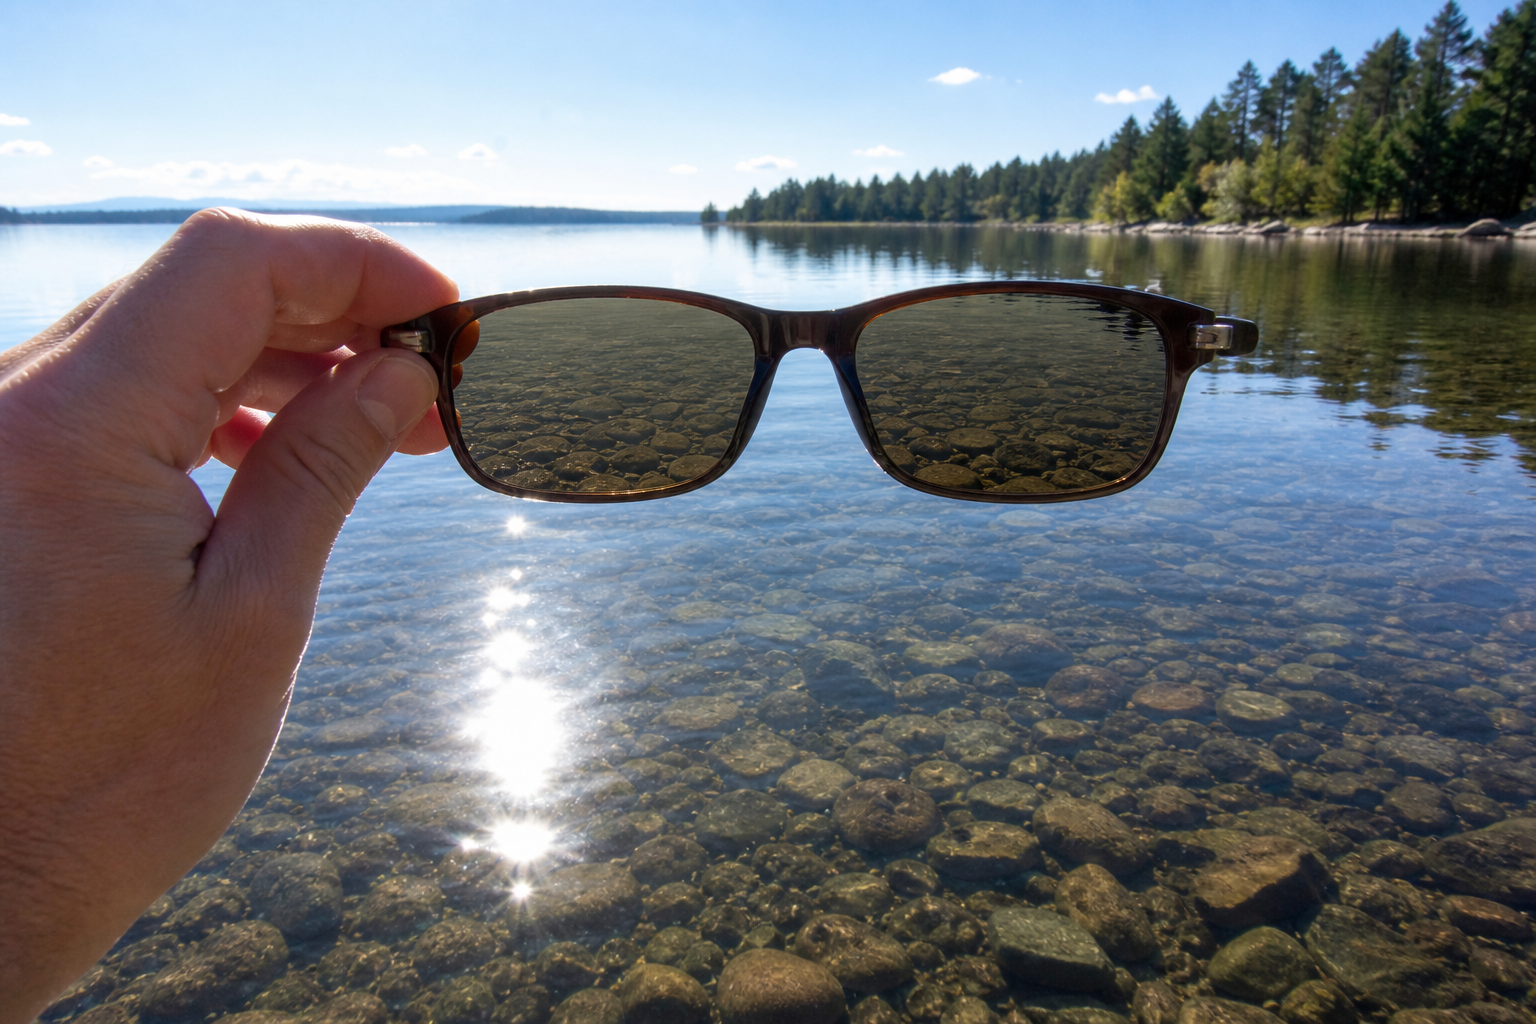
\includegraphics[width=0.58\linewidth]{images/book4/ai/b4-13-polarizing-sunglasses-lake.png}

{\small किसी झील के सामने रखे ध्रुवक धूप-चश्मे: चौंध, जो ब्रूस्टर कोण के पास परावर्तित होकर क्षैतिज ध्रुवित है, लेंसों की ऊर्ध्वाधर पारगमन-अक्ष से कट जाती है, और झील का तल दिखने लगता है।}
\end{omfigure}

\section{समस्या: तरंग, पर्दा और पाल}

\begin{problem}[{सप्ताहांत समस्या --- कोई लेज़र-पुंज अपने क्षेत्रों में
खोला गया, कोई पर्दा जो ध्रुवण से चित्र बनाता है, और कोई अंतरिक्ष-यान जो
प्रकाश पर पाल तानता है}]
\label{pb:b2:plane-waves-polarization:1}

\medskip
\noindent\textbf{भाग I --- पुंज।}
कोई हीलियम--नियोन लेज़र \qty{1.0}{mm} व्यास के पुंज में \qty{632.8}{nm} पर
\qty{10}{mW} देता है, जो $x$ के अनुदिश रैखिक ध्रुवित है और $z$ के अनुदिश
चलता है।
\begin{enumerate}
  \item आवृत्ति, तरंग-संख्या, फ़ोटॉन-ऊर्जा; और प्रति सेकंड उत्सर्जित
        फ़ोटॉन।
  \item तीव्रता; आयाम $E_0$ और $B_0$; तथा $\vect E(z, t)$ और
        $\vect B(z, t)$ लिखिए।
  \item ऊर्जा घनत्व (माध्य) और पुंज के \qty{1}{m} में समाई ऊर्जा;
        \qty{1}{ns} में उत्सर्जित पुंज कितना लंबा है, और उसमें कितनी
        तरंगदैर्घ्य समाती हैं?
  \item \omterm{thm:b2:poynting-vector:poynting}{पॉयनटिंग सदिश}: माध्य मान और उसका दोलन; प्रति सेकंड ढोया गया
        संवेग; और किसी काले लक्ष्य पर तथा किसी दर्पण पर बल।
  \item $E_0$ की उस क्षेत्र से तुलना कीजिए जो किसी हाइड्रोजन परमाणु में
        इलेक्ट्रॉन को बाँधे रखता है (\qty{5e11}{V/m}), और $B_0$ की पृथ्वी के
        क्षेत्र (\qty{50}{\micro T}) से।
  \item किसी काले पुंज-रोधक पर \omterm{prop:b2:poynting-vector:wave}{विकिरण दाब}, पास्कल में।
  \item पुंज में रखा कोई मुक्त इलेक्ट्रॉन: विद्युत क्षेत्र में उसके वेग के
        दोलन का आयाम (पहले चुंबकीय बल छोड़ दीजिए); उस पर चुंबकीय और
        विद्युत बलों का अनुपात --- साधारण प्रकाश में पदार्थ के लिए
        चुंबकीय बल नगण्य क्यों है?
  \item उसी पुंज के क्षेत्र लिखिए यदि वह वृत्तीय
        ध्रुवित होता; तीव्रता में, \omterm{thm:b2:poynting-vector:poynting}{पॉयनटिंग सदिश} में और उसकी
        समय-निर्भरता में क्या बदलता है?
  \item पुंज ऐसे ध्रुवक से गुज़रता है जिसकी अक्ष $x$ से
        \qty{30}{\degree} बनाती है: पार गई शक्ति; फिर पहले से क्रॉस किसी दूसरे
        से: शक्ति; और उनके बीच पहले से \qty{45}{\degree} पर कोई
        तीसरा रखिए: शक्ति।
\end{enumerate}

\medskip
\noindent\textbf{भाग II --- पर्दा।}
कोई द्रव-क्रिस्टल पर्दा: पश्च-प्रकाश (\omterm{def:b2:plane-waves-polarization:states}{प्राकृतिक प्रकाश}), कोई ध्रुवक,
कोष्ठ, और कोई क्रॉस ध्रुवक। बिना वोल्टता के कोष्ठ ध्रुवण को
\qty{90}{\degree} घुमा देता है; और वोल्टता के साथ कुछ नहीं करता।
\begin{enumerate}[resume]
  \item उजली अवस्था में पश्च-प्रकाश की तीव्रता का पार जाता
        अंश (पूर्ण ध्रुवक); और गहरी अवस्था में।
  \item कोई मध्यवर्ती वोल्टता कोष्ठ को अपनी अक्षों के बीच $\delta$ कला का
        कोई मंदक बना देती है, और वे अक्षें ध्रुवकों से \qty{45}{\degree} पर हैं
        (कोई घूर्णन नहीं): दिखाइए कि पारगमन
        $\sin^2(\delta/2)$ है --- यही धूसर मापनी है।
  \item पर्दे के निर्गम ध्रुवक से \qty{90}{\degree} पर घुमाए गए किसी ध्रुवक से
        देखने पर क्या दिखता है? \qty{45}{\degree} पर?
  \item पर्दे पर उसके ध्रुवक से \qty{45}{\degree} पर चिपकाई गई कोई
        \omterm{prop:b2:plane-waves-polarization:plates}{चतुर्थांश-तरंग पट्टिका} निर्गम को वृत्तीय कर देती है: ध्रुवक धूप-चश्मे
        पहने किसी दर्शक के लिए इसका क्या लाभ?
  \item पूर्ण ध्रुवक उजली अवस्था में पश्च-प्रकाश का आधा पार जाने देते;
        पर असली चादरें हर एक आदर्श का $85\%$ पार जाने देती हैं, और
        किसी पिक्सेल की रंग-छन्नियाँ प्रकाश का एक-तिहाई:
        सफ़ेद में दर्शक तक पहुँचती पश्च-प्रकाश की शक्ति का अंश;
        और वे दो जगहें बताइए जहाँ अधिकांश प्रकाश खोता है।
  \item असली क्रॉस चादरें प्रकाश का $0.1\%$ रिसा देती हैं: अँधेरे कमरे में
        पर्दे का विषमता अनुपात (उजला बटा गहरा)।
  \item छायाचित्रकारों के ``वृत्तीय ध्रुवक'' कोई रैखिक ध्रुवक होते हैं
        और उसके बाद \qty{45}{\degree} पर कोई \omterm{prop:b2:plane-waves-polarization:plates}{चतुर्थांश-तरंग पट्टिका}: कैमरा क्या
        पाता है, और वह उसके स्वतः-केंद्रण के ध्रुवण-संवेदी
        पुंज-विभाजक के लिए रैखिक प्रकाश से बेहतर क्यों है?
  \item त्रि-विम सिनेमा के चश्मे रैखिक के बदले \omterm{def:b2:plane-waves-polarization:states}{वृत्तीय ध्रुवण} क्यों
        काम में लेते हैं? यदि दर्शक रैखिक चश्मों के साथ सिर \qty{20}{\degree}
        टेढ़ा कर ले तो दोनों आँखों के बीच रिसाव का
        क्या होता है (ग़लत आँख में रिसती तीव्रता)?
\end{enumerate}

\medskip
\noindent\textbf{भाग III --- पाल।}
$S = \qty{1000}{m^2}$ क्षेत्रफल और कुल द्रव्यमान $m = \qty{50}{kg}$ का कोई सौर पाल,
जो पूरा परावर्तक है, सूर्य से $D = \qty{1.0}{au} = \qty{1.5e11}{m}$ पर
($I = \qty{1.36}{kW/m^2}$; वहाँ सूर्य का गुरुत्व \qty{5.9e-3}{m/s^2})।
\begin{enumerate}[resume]
  \item जब पाल सूर्य के सामने हो तो विकिरण बल; त्वरण;
        और सौर गुरुत्व से अनुपात।
  \item पाल सूर्य के सामने से $\theta$ झुकाया जाता है: दिखाइए कि
        बल पाल के अभिलंब है और $\cos^2\theta$ के समानुपाती
        (रोकी गई शक्ति $\times\cos\theta$, और अभिलंब के अनुदिश संवेग-परिवर्तन
        $\times\cos\theta$)।
  \item बाहर की ओर सर्पिल में जाने के लिए पाल अपने कक्षीय वेग के अनुदिश
        कोई बल-घटक बनाए रखता है: $\theta = \qty{35}{\degree}$ के लिए स्पर्शीय
        त्वरण; प्रति वर्ष पाई गई चाल; और पृथ्वी की
        कक्षीय चाल (\qty{30}{km/s}) से तुलना।
  \item वही पाल बुध ($D = \qty{0.39}{au}$) के पास $6.6$ गुना बल क्यों पाता
        है, और गुरुत्व से उसका अनुपात क्यों नहीं बदलता?
  \item पाल की झिल्ली \qty{2}{\micro m} की ऐलुमिनियम-लेपित प्लास्टिक है: धूप में
        उसका ताप, यदि वह $10\%$ सोखे और दोनों फलकों से
        कृष्णिका की तरह विकिरित करे ($\sigma = \qty{5.67e-8}{W.m^{-2}.K^{-4}}$)।
  \item सूर्य के सामने रहकर \qty{1}{km/s} पाने में लगा समय; और उसी आकार
        का कोई सोखता (काला) पाल क्या पाता?
  \item फ़ोटॉनों से प्रकाश का संवेग जाँचिए: प्रति सेकंड पाल से टकराते
        फ़ोटॉनों की संख्या (औसतन \qty{2}{eV}) और हर एक का
        संवेग $hf/c$; और उससे बल फिर से पाइए।
  \item सार दीजिए: तरंग द्वारा ढोई गई तीन राशियाँ (ऊर्जा,
        संवेग, ध्रुवण) और इस समस्या का वह उपकरण जो हर एक का
        उपयोग करता है।
\end{enumerate}
\end{problem}
